
\documentclass[a4paper,12pt]{article}
\usepackage[spanish]{babel}
\usepackage[utf8]{inputenc}
\usepackage{imakeidx}
\usepackage{graphicx}
\usepackage{float}
\usepackage{amsmath}
\usepackage[backend=bibtex,style=verbose]{biblatex}
\bibliography{bibliography}
\usepackage{csquotes}
\usepackage{tcolorbox}
\usepackage{multirow}
\usepackage{caption}
\usepackage{float}
\begin{document}

\title{Medida de la Constante de Hubble}

\author{Gabriel D'Andrade Furlanetto - XDD204950}
\date{}
\maketitle
\pagebreak

\section{Objetivos}
Utilizando imágenes de galáxias providenciadas por SAO-DDS, se miden los ángulos en los extremos 
de las galáxias y los utilizan para calcular la distancia entre la Tierra y esas galáxias. 
De esta manera, utilizando datos conocidos da la literatura para las velocidades de
recesión y, finalmente, se calcula la constante de Hubble, $H_0 =\frac{v_{rec}}{d}$, para diferentes configuraciones
de los datos (Excluyendo galaxias del tipo \textbf{Sa} y utilizando valor diferente para $D$).

\section{Teoría}

Experimentalmente, se miden dos pares de ángulos para cada galáxia, $(\alpha, \delta)$, 
que corresponden a dar dos vectores unitários en coordenadas polares con centro
en la Tierra y dirección hasta los extremos de la galáxias.

De esta manera, es necesario medirse en ángulo entre estos vectores, que nos dará 
información sobre la distancia entre la Tierra y la galáxia. Para poder calcularlo,
es necesario utilizar la definición del producto escalar (para vectores unitários)
y su cálculo en las coordenadas del problema:
$$\vec{r_1} \cdot \vec{r_2} = \cos(\theta)$$

$$ \cos(\alpha_1)\cos(\alpha_2)\cos(\delta_1)\cos(\delta_2) + \sin(\alpha_1)\sin(\alpha_2)\cos(\delta_1)\cos(\delta_2) + \sin(\delta_1)\sin(\delta_2
) = \cos(\theta)$$

O sea, que:
\begin{equation}
    \label{theta}
    \theta = \arccos(\cos(\alpha_1)\cos(\alpha_2)\cos(\delta_1)\cos(\delta_2) + \sin(\alpha_1)\sin(\alpha_2)\cos(\delta_1)\cos(\delta_2) + \sin(\delta_1)\sin(\delta_2
))
\end{equation}

Pero, por manipulaciones elementales y la aproximación del ángulo pequeño, se puede
afirmar que


\begin{equation}
    \label{d}
    d = \frac{D}{\theta}
\end{equation}

Donde $d$ es la distancia entre la Tierra y la galáxia. O sea, se puede calcular $d$ 
con los parámetros de los ángulos.

\section{Resultados}

Utilizando los datos obtenidos en el servidor de imágenes SAO-DDS para el 
cálculo de los ángulos de separación, los datos de la literatura\footnote{\cite{literatura}}
para las velocidades, tomando $D=20kpc$ como hipótesis y las ecuaciones 
\eqref{theta} y \eqref{d} para calcular d, se puede montar una tabla para los resultados: 
\begin{table}[h!]
    \label{Tabla}
    \caption{Datos experimentales con las distancias de la galáxia a la Tierra y sus velocidades de recesión}

    \hskip-2.5cm
    \begin{tabular}{|l|l|l|l|l|l|l|l|}
    \hline
        Nombre & Tipo & $v_{rec}(km/s)$ & $\alpha_1$ ( °)& $\delta_1$( °) & $\alpha_2$( °) & $\delta_2$( °) &  $d(Mpc)$\\ \hline
        NGC1357 & Sa & 2100 & 53,3049536 & -13,6755980 & 53,3450165 & -13,6482955 & 19,8284181626923 \\ \hline
        NGC1832 & SBb & 1860 & 78,0089999 & -15,6697095 & 78,0118856 & -15,7095330 & 28,7693357835023 \\ \hline
        NGC2276 & Sc & 2650 & 111,7342764 & 85,7412320 & 111,9762775 & 85,7767928 & 4,69744774486586 \\ \hline
        NGC2775 & Sa & 1200 & 101,8265793 & 33,5587375 & 101,8199689 & 33,5751089 & 68,3132392733834 \\ \hline
        NGC2903 & Sc & 470 & 143,0006753 & 21,4390048 & 143,0833311 & 21,5827808 & 7,79875407904869 \\ \hline
        NGC3034 & I0 & 410 & 149,1632762 & 69,7157523 & 148,7589930 & 69,6423744 & 2,96748555550789 \\ \hline
        NGC3147 & Sb & 2900 & 154,2000000 & 73,3809531 & 154,1433262 & 73,4230137 & 16,6813470349056 \\ \hline
        NGC3227 & Sb & 1100 & 155,8925518 & 19,8360856 & 155,8623463 & 19,8886482 & 21,3969440902952 \\ \hline
        NGC3245 & S0 & 1210 & 156,8247937 & 28,5258558 & 156,8293384 & 28,4898004 & 31,7247221187108 \\ \hline
        NGC3310 & Sbc & 1070 & 159,7074635 & 53,4890406 & 159,6797433 & 53,5219247 & 28,8471760475822 \\ \hline
        NGC3368 & Sab & 760 & 161,6665901 & 11,8566713 & 161,7120194 & 11,7871466 & 16,3364087121769 \\ \hline
        NGC3417 & Sa & 2140 & 162,7503313 & 8,4727266 & 163,7628212 & 8,4755998 & 7,67886943013609 \\ \hline
        NGC3516 & S0 & 2840 & 166,6732804 & 72,5599498 & 166,7213403 & 72,5771988 & 23,3908664560281 \\ \hline
        NGC3623 & Sa & 680 & 169,7405912 & 13,0272327 & 169,7244857 & 13,1627615 & 8,45208171274172 \\ \hline
        NGC3627 & Sb & 590 & 170,0644892 & 12,9251441 & 170,0639776 & 13,0429274 & 9,7290111977366 \\ \hline
        NGC3941 & SB0 & 940 & 178,2251883 & 36,9652890 & 178,2351670 & 37,0074966 & 26,8789746819473 \\ \hline
        NGC4472 & S0 & 820 & 187,4659656 & 7,9527361 & 187,4301237 & 8,0522163 & 11,5045695347057 \\ \hline
        NGC4631 & Sc & 610 & 190,6386176 & 32,546125 & 190,4052701 & 32,5296233 & 9,05234602799548 \\ \hline
        NGC4775 & Sc & 1380 & 193,4547332 & -6,6101842 & 193,4277089 & -6,6313634 & 53,5295254111754 \\ \hline
        NGC5248 & Sbc & 1050 & 204,4035176 & 8,8627666 & 204,3697763 & 8,9100830 & 24,0725349055653 \\ \hline
        NGC5548 & Sa & 4960 & 214,5099643 & 25,1385214 & 214,4818249 & 25,1378162 & 95,696534407399 \\ \hline
        NGC5866 & S0 & 820 & 226,6644517 & 55,7443765 & 226,5821534 & 55,7833323 & 14,6160554648118 \\ \hline
        NGC6181 & Sc & 2440 & 248,0894849 & 19,8052821 & 248,0824229 & 19,8448563 & 28,9032427161406 \\ \hline
        NGC6217 & SBbc & 1600 & 248,1218207 & 78,2132040 & 248,1956674 & 78,1824260 & 14,5855420686077 \\ \hline
        NGC6643 & Sc & 1740 & 275,0116358 & 74,5877849 & 274,8840190 & 74,5491538 & 8,8872540353652 \\ \hline
        NGC6764 & SBb & 2410 & 287,0951042 & 50,9406932 & 287,0448228 & 50,9268493 & 27,6648634818234 \\ \hline
        NGC7469 & Sa & 5120 & 345,8192889 & 8,87000973 & 345,8105057 & 8,877936 & 142,504839944925 \\ \hline
    \end{tabular}
\end{table}

Como se había mencionado antes, se tiene interés en determinar la relación entre la velocidad de recesión, $v$, y la
distancia de la Tierra, $d$. Representándo-lo gráficamente (figura \ref{fig:H1}) y utilizando las herramientas de LibreOffice Calc para
automáticamente calcular la regresión lineal por el método de mínimos cuadrados, se tiene que:
$$H_{01} = 43 km/s Mpc$$

Con mínimas alteraciones, se puede hacer la análisis que excluye los datos de tipo \textbf{Sa}, 
representarla gráficamente (figura \ref{fig:H2}), y obtener el valor para la constante de Hubble de la ecuación dada para estos datos:
$$H_{02} = 58 km/sMpc$$  

Finalmente, se puede hacer lo mismo utilizando $D=10kpc$ (figura \ref{fig:H3}) y obtener la constante de Hubble para
este conjunto:
$$H_{03} = 86 kpc$$

\begin{figure}[H]
    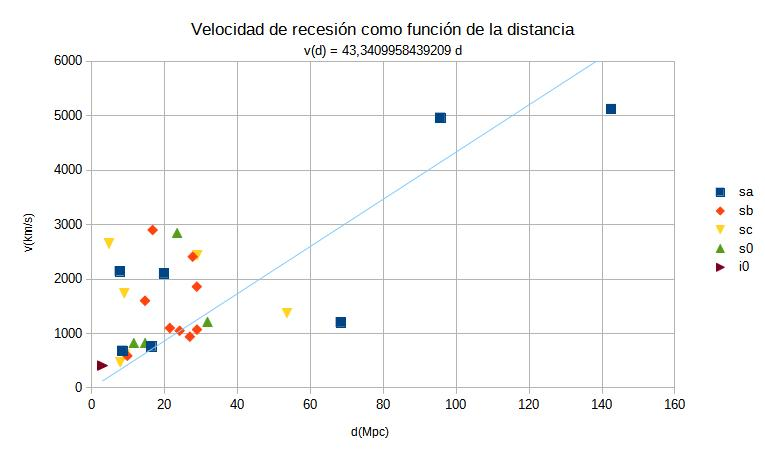
\includegraphics[width=\textwidth]{g1.jpg}
    \caption{Gráfico de los valores obtenidos de $d$ para los diferentes valores de $v$. Se tiene puesta ecuación de la regresión lineal obtenida.}    
    \label{fig:H1}
\end{figure}

\begin{figure}[H]
    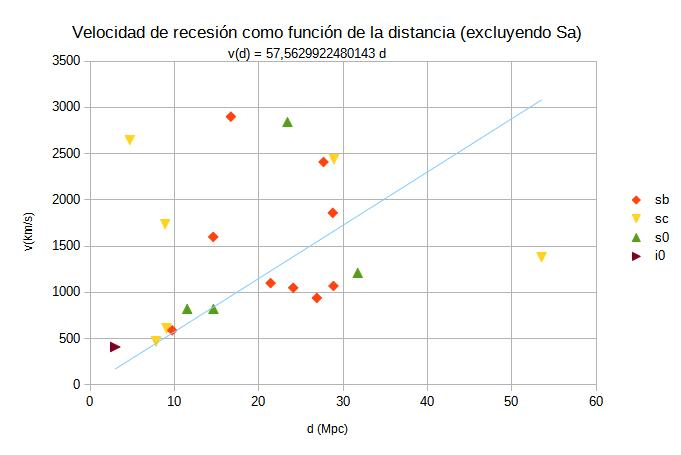
\includegraphics[width=\textwidth]{g2.jpg} 
    \caption{Gráfico de los valores obtenidos de $d$ para los diferentes valores de $v$ excluyendo galáxias de tipo \textbf{Sa}.}    
    \label{fig:H2}
\end{figure}

\begin{figure}[H]
    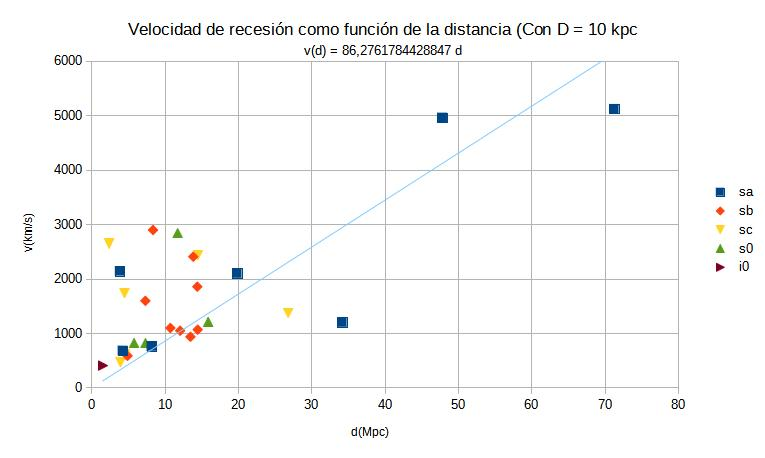
\includegraphics[width=\textwidth]{g3.jpg}
    \caption{Gráfico de los valores obtenidos de $d$ para los diferentes valores de $v$ tomando $D=10kpc$.}
    \label{fig:H3}
\end{figure}



\section{Análisis y Conclusión}

Utilizando el valor de la literatura\footnote{\cite{hubble}} como referencia, $H_0 = 73 km/s Mpc$,
se pueden analizar los resultados obtenidos. Primeramente, es posible concluir que todos los
resultados están distantes del de la literatura. Más precisamente, tenemos un error relativo de
$\epsilon_n = \left| \frac{H_{0n}-H_{0}}{H_0}\right|$

    $$\epsilon_1 = 0.4109 = 41.09\%$$
    $$\epsilon_2 = 0.2054 = 20.54 \%$$ 
    $$\epsilon_3 = 0.1780 = 17.80 \%$$ 


Esto se debe, principalmente, a dos factores: Primeramente, a la falta de precisión en calcular 
$\alpha$ y $\delta$, que indubitablemente no fueron obtenidas de la manera más sistemática 
(con mucha discreción humana). Más allá, se tiene que considerar que, obviamente, los tamaños 
de las galáxias, $D$, no son constantes, y esto obviamente se traduce en valores menos precisos.

No obstante a estos problemas, se ha podido alcanzar los objetivos iniciales de manera satisfactoria 
y producir resultados aceptables en los parámetros en que se trabajaba.

\printbibliography
\end{document}
